\title{Labo: Ontwerp van een audio versterker}
\author{}
\date{}

\documentclass{article}
	\usepackage[a4paper]{geometry}
	%\usepackage[utf8x]{inputenc}
	\usepackage[T1]{fontenc}
	\usepackage[dutch]{babel}
	\usepackage{amsmath}
	%%% FIGURES %%%
	\usepackage[pdftex]{graphicx}
	\usepackage{caption,subcaption}
	\usepackage{hyperref}
	\graphicspath{ {./figs/} }

\begin{document}
\maketitle
\begin{figure}[htbp]
	\centering
	\includegraphics[width=0.4\textwidth]{foto.jpg}
	\caption{E-VUBOX 2k15}
	\label{fig:foto}
\end{figure}

\tableofcontents

\section{Doelstelling}
In dit labo gaan we een eerste stap in de elektronica zetten door zelf een audio versterker te maken, stap voor stap van de basiselektronica tot het finaal product. Tijdens deze opdracht gaan we ook een kijkje nemen in het brein van een ingenieursstudent elektronica wanneer die zo'n taak vervuld. 
We gaan beginnen met een inleiding in de elektronica, kennismaking met basisregels, componenten en schakelingen, naar complexere onderdelen, tot de versterker!

Elektronica kan interessant zijn om te bestuderen omdat veel leuke en/of nuttige objecten mogelijk zijn omwille van elektronica. Alledaagse objecten zoals een GSM of een computer bevatten veel elektronica. In de ziekenhuis kan je ook allerhande toestellen vinden die dagelijkes levens redden. In de entertainment wereld vind je elektronica terug in cameras, schermen en spelconsoles. Veel geavanceerde objecten zoals zelfrijdende autos, vliegtuigen, straaljagers en automatische robots in fabrieken zouden niet mogelijk zijn zonder de elektronica. 


Als stromen, spanningen, de wet van Ohm en de wetten van Kirchhoff geen bekende concepten zijn, volgt hier een overzicht van de wonderlijke wereld van de elektronica met alles wat je moet weten. Indien je al een basis hebt in elektronica, mag je het deel ``Elektronica: componenten en schakelingen'' snel overlopen en onmiddellijk beginnen met hoofdstuk \ref{sec:bouwstenen} op pagina \pageref{sec:bouwstenen}. 

\section{Elektronica: componenten en schakelingen}
Elektronica is het gebruik van de beweging van elektronen om informatie te verwerken, te versturen of op te slaan. Dit doen we door netwerken van elektronische componenten te bouwen. Elektronische componenten zijn eenvoudige bouwstenen waarmee we complexe schakelingen kunnen bouwen op zo een manier dat die specifieke taken uitvoeren: het ontvangen en versturen van berichtjes met een gsm, het afbeelden van een foto op een scherm en vele andere toepassingen die je elke dag tegenkomt. Je hebt waarschijnlijk een stuk elektronica in jouw broekzak op dit ogenblik!

De schematische voorstelling van elektronische componenten en een netwerk zijn te vinden in Figuur \ref{fig:component_en_schakeling}. Met pijltjes zijn de twee grootheden aangeduid die in de elektronica opperbelangrijk zijn :

\begin{enumerate}
	\item de \textbf{spanning} (ook voltage of potentiaal genoemd) gemeten in volt [V], vaak aangeduid met de letter $V$ of $U$. Dit stelt het verschil in potenti�le elektrische energie \textbf{tussen twee punten} \footnote{Je kent al een maat voor het verschil in potienti�le gravitationele energie: de hoogte in meter. Zoals een bal valt van hoog naar laag, gaat een positieve lading lopen van een hoge spanning naar een lage spanning.}.
	\item de \textbf{stroom} gemeten in amp�re [A], vaak aangeduid met de letter $I$. Dit stelt de verplaatsing voor van een hoeveelheid ladingen (hier elektronen) door de component per tijdseenheid.
\end{enumerate}

Stroom en spanning veranderen meestal in functie van de tijd, anders zou er natuurlijk niet veel interessants gebeuren, ze worden dan beschreven door wiskundige functies. Enkele voorbeelden:
\begin{align}
     I(t) = 0.1 \text{A} \cdot sin(t), \\
     V(t) = 4 \text{V} \cdot e^{-\frac{t}{10 s}}.
 \end{align} 
 waar $t$ de tijd is in seconden.

\begin{figure}[hbtp]
	\centering
	\begin{subfigure}[b]{0.45\linewidth}
		\centering
		\includegraphics[width=0.8\linewidth]{componenten}
		\caption{Elektronische componenten: een weerstand links en een diode rechts. Men spreekt van de spanning $V$ \textbf{over} de pinnen (1 en 2), en de stroom $I$ \textbf{door} de component. Let op: de zin van de pijlen heeft belang!}
		\label{subfig:componenten}
	\end{subfigure}
	~
	\begin{subfigure}[b]{0.45\linewidth}
		\centering
		\includegraphics[width=0.8\linewidth]{weerstandsdeler}
		\caption{Elektronisch netwerk: een schakeling van componenten. Er is \textbf{over} elk component een spanningsval , en \textbf{door} elk component een stroom.}
		\label{subfig:netwerk}
	\end{subfigure}
	\caption{Componenten en een schakeling. }
	\label{fig:component_en_schakeling}
\end{figure}
 Elke component voldoet aan fysische wetten die zijn stroom en de spanning bepalen. Laten we kennismaken met die fysische wetten, en daarna we gaan onmiddellijk ons eerste netwerk oplossen. We bekijken twee basiselementen van de elektronica: de weerstand en de spanningsbron.

\subsection{De weerstand}

In figuur \ref{subfig:componenten} zie je de schematische voorstelling van een weerstand. Een weerstand is een geleider die voldoet aan de \textbf{wet van Ohm}: 
\begin{align}
	V &= R \cdot I
\end{align} 
$R$ is een eigenschap van de  weerstand die men ook elektrische weerstand noemt, het is gemeten in Ohm\footnote{Georg Simon Ohm (1787 - 1854) was een Duits wiskundige en natuurkundige, ontdekker van de wet van Ohm in 1827.} [$\Omega$]. $V$ is de spanning over de weerstand en $I$ de stroom door de weerstand.

Een weerstand kan je zien als een belemmer van stroom: om door een grote weerstand een hoge stroom te laten vloeien moet je een grote spanning aanleggen. Met een kleine weerstand voldoet een kleine spanning om een grote stroom te hebben. 

Zo dadelijk volgt een voorbeeld, we gaan eerst zien wat weerstanden in serie en in parallel zijn, en kennismaken met de spanningsbron.

\subsubsection{Serie en parallel}
\label{sssec:serie_en_parallel}
Soms kan je twee weerstanden door een weerstand vervangen als ze speciaal samenzitten, dat kan het ontwerpen gemakkelijker maken. Dit kan in twee gevallen (zie figuur \ref{fig:serie_en_parallel}):

\begin{itemize}
	\item twee weerstanden zijn \textbf{in serie}: ze hebben ��n gemeenschappelijke pin, en dezelfde stroom vloeit door de twee weerstanden, dan is de vervangingsweerstand :
	\begin{align}
		R_{v} = R_1 +R_2.
	\end{align}
	Door weerstanden in serie te plaatsen, krijg je dus een grotere weerstand.

	\item twee weerstanden staan \textbf{parallel}: de twee weerstanden hebben beide pinnen gemeenschappelijk, dus de spanning over de twee is dezelfde. Dan geldt voor de vervangingsweerstand 
	\begin{align}
		\frac{1}{R_{v}}= \frac{1}{R_{1}} + \frac{1}{R_{2}} 
	\end{align}
	Door weerstanden in parallel te plaatsen, krijg je een kleine weerstand.
\end{itemize}

\begin{figure}[hbtp]
	\centering
	\begin{subfigure}[b]{0.45\linewidth}
		\centering
		\includegraphics[width=0.5\linewidth]{serie}
		\caption{Weerstanden in serie.}
		\label{subfig:serie}
	\end{subfigure}
	~
	\begin{subfigure}[b]{0.45\linewidth}
		\centering
		\includegraphics[width=0.8\linewidth]{parallel}
		\caption{Weerstanden in parallel.}
		\label{subfig:parallel}
	\end{subfigure}
	\caption{Serie en parallel.}
	\label{fig:serie_en_parallel}
\end{figure}

\subsection{De spanningsbron}

\begin{figure}[htbp]
	\centering
	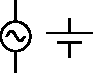
\includegraphics[width=0.1\textwidth]{spanningsbron.pdf}
	\caption{Spanningsbronnen. Links: de spanning verandert met de tijd. Rechts: de spanning is constant.}
	\label{fig:vbron}
\end{figure}

 Een spanningsbron is een simpel elektronisch component die gehoorzaamt aan een eenvoudige wet: de spanningsbron legt de spanning over zijn pinnen vast, onafhankelijk van de rest van het netwerk. Een 9V-batterij is een voorbeeld van een spanningsbron, die de spanning over zijn pinnen vastlegt op constant $9~V$. Een spanningsbron kan een constante spanning opleggen, maar niets verbiedt dat de spanning met de tijd verandert. Beide type bronnen hebben hun eigen schematische voorstelling die je kan vinden in figuur \ref{fig:vbron}.

\subsection{Mini-netwerk}
We gaan binnenkort wetten ontdekken van nog meer componenten, maar met onze voorlopige kennis kunnen we al volgend netwerk oplossen!
\paragraph*{Voorbeeld:} 
\begin{figure}[h!]
	\centering
	\includegraphics[width=0.25\textwidth]{vbweerstand.pdf}
	\caption{Voorbeeldnetwerkje.}
	\label{fig:vbweerstand}
\end{figure}

Een spanningbron legt en spanning op van $50~V$ over een weerstand van $200~\Omega$. Men kan de stroom door de weerstand berekenen op de volgende manier:

\begin{align}
	\text{(Wet van Ohm)}~V = R\cdot I \Leftrightarrow I = \frac{V}{R} \Leftrightarrow I = \frac{50~V}{200~\Omega}= 0,25~A
\end{align}

\paragraph*{Doe-het-zelf:} Wat is de waarde $R$ van een weerstand waarover een spanning van $V = 25~V$ is en waardoor een stroom van $I = 0.1~A$ loopt?
\\.\dotfill \\.\dotfill \\.\dotfill 

Nu we een simpel netwerk kunnen oplossen, gaan we zien hoe we grotere netwerken moeten oplossen.
\subsection{Netwerken}
Een netwerk is een aaneenschakeling van componenten, die schematisch wordt voorgesteld zoals in figuur \ref{subfig:netwerk}. Er zijn maar twee regels die gelden voor elektrische netwerken: de wetten van Kirchhoff\footnote{Gustav Robert Kirchhoff (1824 - 1887) was een Duits natuurkundige. Kirchhoff formuleerde zijn spanningswet en zijn stroomwet in 1845, toen hij nog een student was. Slimme kerel!}. Samen met de fysische wetten van de componenten kan je dan alle netwerken van de wereld oplossen. Een netwerk oplossen wilt zeggen dat je alle stromen en spanningen bepaalt in dat netwerk.

\paragraph*{De stroomwet van Kirchhoff:} in elk knooppunt in een elektrische kring is de som van de stromen die in dat punt samenkomen gelijk aan de som van de stromen die vanuit dat punt vertrekken. Dit is voor elk knooppunt geldig, onafhankelijk van de componenten die op de takken zijn. 
\paragraph*{De spanningswet van Kirchhoff:} de som van de elektrische potentiaalverschillen (rekening houdend met de richting) in elke gesloten lus in een kring is gelijk aan nul. 

\paragraph*{Voorbeeld}
De stroomwet (figuur \ref{subfig:kcl}) wordt toegepast als volgt: kies een knooppunt in een netwerk. Beschouw alle takken die dat knooppunt raken, en de bijhorende stromen. Pas op, de richting van de stroom-pijlen is zeer belangrijk. Als je alle stromen optelt die \textbf{naar} het knooppunt wijzen, dan is dat gelijk aan alle stromen die \textbf{weg} van het knooppunt wijzen.

\paragraph*{}
Voor dat we spanningswet toepassen, hebben we de betekenis van het symbool \includegraphics[height=1em]{gnd.pdf} nodig. Dit symbool wordt de \textbf{grond} genoemd. Het is geen component, maar een manier aan te duiden dat alle punten met dat symbool eigenlijk verbonden zijn. Je mag dus eigenlijk een connectie tekenen tussen alle pinnen die aan de grond verbonden zijn. Er werd al gezegd dat een spanning altijd gedefinieerd is tussen twee punten. Meestal wordt de grond gebruikt als een van die twee punten, en we zeggen dat de grond op 0 V is.

\paragraph*{Voorbeeld}
De spanningswet (figuur \ref{subfig:kvl}) pas je zo toe: vind een gesloten lus in het netwerk (vergeet niet dat alle pinnen aan grond met elkaar verbonden zijn). Teken een lus met een zekere richting in het netwerk. Schrijf de som van de spanningen rekening houdend met de volgende regels:

\begin{enumerate}
 	\item Als de spanning in dezelfde richting gaat als de lus, dan krijgt die een positief teken.
 	\item Als de spanning tegen de lus ingaat, dan krijgt die een negatief teken.
 \end{enumerate}

\begin{figure}[htbp]
	\centering
	\begin{subfigure}[b]{0.45\linewidth}
		\centering
		\includegraphics[width=0.7\textwidth]{kcl.pdf}
		\caption{In dit knooppunt is de stroomwet van Kirchhoff : $i_1 + i_4 = i_2+i_3$}
		\label{subfig:kcl}
	\end{subfigure}
	~
	\begin{subfigure}[b]{0.45\linewidth}
		\centering
		\includegraphics[width=0.8\textwidth]{kvl.pdf}
		\caption{In deze lus is is de spanningswet van Kirchhoff : $ + V_S - V_1 - V_2 = 0$}
		\label{subfig:kvl}
	\end{subfigure}
\caption{De wetten van Kirchhoff}
\label{fig:kirchoff}
\end{figure}

\paragraph*{Fun fact:} Je kan de vergelijkingen voor serie en parallel weerstanden (sectie \ref{sssec:serie_en_parallel}) afleiden met behulp van de wetten van Kirchoff en de wet van Ohm.

\paragraph*{Oefening van Kirchhoff:}
- 4 takken met ��n onbekende: KCL
- lus met 5 componenten met ��n onbekende spanning: KVL

We zijn nu gereed om de bouwstenen van onze versterker te ontwerpen!

\section{Bouwstenen van de E-VUBOX}
\label{sec:bouwstenen}
In dit deel gaan we stap voor stap de onderdelen van onze versterker bouwen. We beginnen met een volumeregelaar, omdat we alles al kennen om die te maken. We gaan dan een simpele aan/uit LEDje ontwerpen zodat we weten wanneer onze versterker aan is. Daarna houden we ons bezig met de eigenlijke versterking en gaan we kennismaken met de transistor die ons daarmee gaat helpen. 

Maar eerst en vooral: waarom en hoe versterk je muziek?

\subsection{Versterken van audio}

Ook als je een student in elektronisch ingenieur bent, is een basiskennis in de rest van de wetenschappen toch handig. Want voordat we geluid gaan versterken, moeten we weten wat geluid is!

Geluid is een drukgolf door een lucht. De luchtdeeltjes bewegen heen en weer, en wanneer ze jouw trommelvlies raken, hoor je het geluid. Om het te versterken moeten we eerst de drukgolf omzetten naar iets dat een elektronisch schakeling kan gebruiken. Daarvoor dient een microfoon! Het trillen van luchtdeeltjes wordt in een microfoon omgezet naar het trillen van elektronen. Voor de rest van het netwerk is de microfoon eigenlijk een spanningsbron.

Een voorbeeld van een specifiek geluid is een muzieknoot. De muzieknoot ``la'' hoor je wanneer de luchtdruk op een zekere plaats golft met een frequentie\footnote{frequentie is het aantal volledige golven (op en neer) per seconde} van $440$ Hz. Je kan de luchtdrukgolf die we horen als een ``la'' wiskundig voorstellen als een sinus:

\begin{align}
	y(t) = A \cdot \sin (2\pi \cdot 440~\text{Hz} \cdot t)
\end{align}

met $y(t)$ de luchtdruk in Pascal, $A$ de amplitude van de drukgolf in Pascal en $t$ de tijd in seconden.

De microfoon gaat die drukgolf omvormen naar een spanningsgolf, met dezelfde frequentie (zie figuur \ref{fig:micro}. Men kan die nu versterken met een elektronisch netwerk, omdat we een spanning hebben! Die spanningsgolf kan dan onmiddelijk worden versterkt of opgeslagen in een mp3-bestand en later gebruikt in een muziekspeler.

\begin{figure}[htbp]
	\centering
	\includegraphics[width=0.95\textwidth]{micro}
	\caption{Een microfoon vormt de luchtdrukgolf (eenheid: Pascal) om in een spanningsgolf (eenheid: Volt).}
	\label{fig:micro}
\end{figure}

Om de muziek te kunnen horen moeten we de spanningsgolf terug omzetten naar een luchtdrukgolf, en daarvoor gebruiken we een luidspreker, die exact het omgekeerde doet van een microfoon. Maar als we de spannigsgolf onmiddelijk aansluiten aan de luidspreker, gaat het geluid zeer zeer stil zijn. We komen eindelijk in de kern van dit project: het geluidssignaal moet versterkt worden!

Inderdaad, de luidspreker heeft meer `schwung' nodig om luid muziek af te spelen. Om dat te doen moeten we het \textbf{elektrisch vermogen} over de luidspreker groot houden. Het elektrisch vermogen dat een component verbruikt wordt berekend als volgt:
\begin{align}
     P = V \cdot I
     \label{eq:vermogen}
 \end{align} 

 met $P$ het vermogen in Watt, $V$ het voltage over de component en $I$ de stroom door de component. We moeten door de luidspreker dus veel stroom en een hoge spanning aanleggen (X). Dat is net de bedoeling van een versterker.

Nu dat we weten waarom onz netwerk nuttig is, kunnen we aan de bouw van onze versterker beginnen!

\subsection{De volumeknop: de spanningsdeler}

We hebben de muziek dus omgevormd naar een spannings-signaal. Stel dat $V_s$ ons muzieksignaal is, en dat we in serie met die spanningsbron twee weerstanden schakelen (figuur \ref{fig:volume}), dan hebben we een zogenaamde \textbf{spanningsdeler} gebouwd. We gaan aantonen de spanning $V_2$ een verkleinde versie is van het muzieksignaal $V_s$. Dit is handig als het geluid te luid is, en dat we het volume willen regelen.

\begin{figure}[htbp]
	\centering
	\includegraphics[width=0.3\textwidth]{weerstandsdeler}
	\caption{Volumeregeling: de spannignsdeler}
	\label{fig:volume}
\end{figure}

Met de stroomwet van Kirchhof kunnen we zien dat alle stromen in het circuit gelijk zijn ($I_s = I_1 = I_2$). We kunnen die stroom berekenen door twee weerstanden de vervangen door hun serie-weerstand, en de stroom door de serieweerstand uit te drukken:

\begin{align}
I_2 = \frac{V_s}{R_1+R_2}	
\end{align}

We gebruiken dan de wet van Ohm om $V_2$ te vinden:
\begin{align}
    V_2 = R_2 \cdot I_2 = \frac{R_2}{R_1+R_2}V_s
\end{align}

Je kan zien dat de spanning $V_2$, die we de uitgangsspanning noemen, altijd kleiner is dan (of gelijk aan) de ingangsspanning $V_s$. Daarom noemen we dit een spanningsdeler.
\paragraph*{Doe-het-zelf:} Je heb een voltage van $9$ V als ingangspanning, en je wilt een voltage van $1.5$ V als uitgangspanning. $R_1$ is al gekozen en heeft een weerstand van $1$ k$\Omega$ ($1000 \Omega$). \marginpar{waardes gebruiken die later nuttig gaan zijn voor transistor.} Welke waarde moet je kiezen voor $R_2$?
\\.\dotfill \\.\dotfill \\.\dotfill \\.\dotfill \\

In de praktijk wordt een spanningdeler vaak met een regelbare weerstand gemaakt (zie figuur \ref{subfig:regelbareR}), zodat de verhouding tussen de in- en uitgangsspanning kan veranderd worden. In figuur \ref{subfig:pot} zie je een \textbf{potentiometer}, dat is een regelbare spanningsdeler. Het is eigenlijk een regelbare weerstand die je in het midden kan aftakken, en dat vormt een spanningsdeler omdat boven de aftakking een weerstand is, en eronder ook.

We gaan een potentiometer gebruiken als volumeknop! Omdat je een potentiometer volledig kunt toedraait of opendraaien, maak de grootte van de weerstand niets uit voor de spannigsverhouding, je kan van een verhouding van 0 tot 1 gaan. Maar wat wel belangrijk is, is dat er niet te veel stroom door de potentiometer vloeit, want anders wordt er vermogen gebruikt door de volumeknop en gaan onze batterij zeer snel plat zijn. 

\paragraph*{Doe-het-zelf:} Welke grootte moet de potentiometer hebben, wetend dat de ingangsspanning $200$ mV is en we het vermogen willen beperken to 4 $\mu$W ( = $4 \cdot 10^{-6}$ W)? \textbf{Tip:} De formule voor elektrisch vermogen kan je vinden op pagina \pageref{eq:vermogen}.
\\.\dotfill \\.\dotfill \\.\dotfill \\.\dotfill \\

En zo is onze eerst deel van onze versterker ontworpen! Laten we verder gaan met de aan/uit knop, zodat we snel naar de versterking kunnen gaan.
\begin{figure}
	\centering
	\begin{subfigure}[b]{0.45\linewidth}
		\centering
		\includegraphics[width=0.5\textwidth]{regelbareR}
		\caption{Spanningsdeler met een regelbare weerstand (weerstand met een pijltje).}
		\label{subfig:regelbareR}
	\end{subfigure}
	~
	\begin{subfigure}[b]{0.45\linewidth}
		\centering
		\includegraphics[width=0.8\textwidth]{potentiometer.pdf}
		\caption{Spanningsdeler met een potentiometer.}
		\label{subfig:pot}
	\end{subfigure}
\caption{Types spanningsdelers.}
\label{fig:vdeler} 
\end{figure}

\subsection{De aan/uit LED: de diode}
Een handig onderdeel op veel elektronische toestellen is het LED-lampje dat brandt om aan te geven dat het toestal aan is. LED staat voor Light Emitting Diode, lichtgevende diode\footnote{Er bestaan ook niet-lichtgevende diodes.}. Laten we eens kennismaken met de diode\ldots 
Een diode (figuur \ref{fig:diode}) is een heel belangrijke en nuttige elektronische component, die alleen stroom doorlaat in ��n richting.
\begin{figure}[htbp]
	\centering
	\includegraphics[width=0.1\textwidth]{diode}
	\caption{Een diode met voorwaarte spanning $U_d$ en stroom $I_D$. De diode laat alleen stroom toe in de  positieve stroomriching (richting van de stroompijl).}
	\label{fig:diode}
\end{figure}

Wanneer een stroom loop door de diode, ontstaat een voorwaarte spanning over de diode. In figuur \ref{fig:diode_grafiek} zie de grafiek van de stroom in functie van de spanning van de diode de we gaan gebruiken in onze versterker. In tegenstelling met de weerstand is de fysische wet van de diode niet-linear (= het is geen rechte), het is een exponenti�le functie.

\begin{figure}[htbp]
	\centering
	\includegraphics[width=0.3\textwidth]{diode_grafiek}
	\caption{Grafiek van de stroom in functie van de spanning van een diode.}
	\label{fig:diode_grafiek}
\end{figure}

Omdat rekenen met een exponenti�le functie onhandig is, gaat een ingenieursstudent meestal eerst proberen om zich te redden met alleen de grafiek. We gaan een circuit oplossen zonder de die moeilijke functie te gebruiken.

\begin{figure}[htbp]
	\centering
	\includegraphics[width=0.5\textwidth]{diode_netwerk}
	\caption{Diode netwerk.}
	\label{fig:diode_netwerk}
\end{figure}
\marginpar{verander i2 door iR}

\begin{itemize}
	\item 20 mA omdat leuk lichtje
	\item komt overeen met 2.1 V
	\item moeten we zorgen dat rest van spanning over weerstand
	\item bereken de weerstand die nodig is.
\end{itemize}

\subsection{De versterker: de transistor}

% \section{Het nut van een versterker}

% Het doel van ons project is om een versterker te bouwen, maar waarom een versterker nodig is wordt hier kort uiteengezet. We willen muziek dat uit onze muziekspeler komt beluisteren. Meestal doen we dat met oortjes of een koptelefoon als we alleen zijn. Maar als we de muziek willen laten beluisteren door vrienden, dan moet het geluid een beetje luider.

% Een luidspreker onmiddellijk aansluiten aan onze muziekspeler gaat geen luid lawaai maken. Dit is omdat een luidspreker een hogere spanning en stroom nodig heeft dan wat de muziekspeler kan geven. Dit is waarom een versterker nuttig is, het gaat de spanning aan de uitgang van de muziekspeler versterken en meer stroom kunnen leveren aan de uitgang.

% \textbf{Uitleg hoe een luidspreker werkt + muziek is een sinus?}

% We weten alles wat nodig is, aan de slag!

% \section{Ontwerp}

% We gaan nu beginnen met het ontwerp, dat bestaat uit het ingenieus kiezen van de elektronische componenten waaruit de versterker is opgebouwd. Die keuze wordt bepaald door de eisen die we hebben voor de versterker:

% \begin{enumerate}
% 	\item Het ontwerp moet eenvoudig zijn.
% 	\item De versterker moet draagbaar zijn, om het overal te kunnen gebruiken. ($\rightarrow$ dwz: batterij)
% 	\item Amplitude van het voltage aan de uitgang van de versterker moet vijf keer groter zijn dan aan de ingang.
% 	\item De uitgang van de versterker moet genoeg stroom leveren om de luidspreker aan te sturen.
% \end{enumerate}

% Enkele elektronische ingenieurs zijn ons voorgeweest en hebben al een elektronisch netwerk gemaakt die aan de eisen kan voldoen. Dat netwerk kunnen we vinden in figuur~\ref{fig:volledig_schema}. Dit is een typisch schema dat elektronische ingenieurs gebruiken. 

% \begin{figure}[htbp]
% 	\centering
% 	\includegraphics[width=\textwidth]{volledig_schema}
% 	\caption{Het gebruikt netwerk voor ons ontwerp.}
% 	\label{fig:volledig_schema}
% \end{figure}





% \begin{itemize}
% 	\item serie
% 	\item parallel
% \end{itemize}

% \paragraph*{Ons eerst netwerk: de weerstandsdeler}

% \begin{itemize}
% 	\item stroom door R1+R2
% 	\item spanning over R2
% 	\item $V_{R2} = \frac{R1}{R1+R2}V$
% \end{itemize}
% \subsection{Jogging: LED}
% \subsection{Eerste Marathon: De Transistor}
% \subsection{Tweede Marathon: De Opamp}


\end{document}